\documentclass[utf8]{frontiersSCNS}
\usepackage{gensymb}
\usepackage{url,hyperref,lineno,microtype,subcaption}
\usepackage[onehalfspacing]{setspace}

\linenumbers
\usepackage{wasysym} % provides \DH, \dh, \Thorn, \thorn
% Leave a blank\usepackage{amsmath}
%\DeclareMathOperator{\sign}{sign} line between paragraphs instead of using \\

\usepackage{booktabs}
\usepackage{multirow}
\usepackage{siunitx} %for SI units

\def\keyFont{\fontsize{8}{11}\helveticabold }
\def\firstAuthorLast{Balasubramanian {et~al.}} %use et al only if is more than 1 author
\def\Authors{Suryanarayanan Balasubramanian\,$^{1}$, Martin Hoelzle\,$^{1}$}
\def\Address{$^{1}$University of Fribourg, Department of Geosciences, Fribourg, Switzerland\\} \def\corrAuthor{Suryanarayanan Balasubramanian}

\def\corrEmail{suryanarayanan.balasubramanian@unifr.ch}


\begin{document}
\onecolumn
\firstpage{1}

\title[Artificial Ice Reservoirs]{Optimal discharge rates for artificial ice reservoir (Icestupa) evolution}

\author[\firstAuthorLast ]{\Authors}
\address{}
\correspondance{}

\extraAuth{}

% \maketitle
\begin{abstract}
  Since 2014, mountain communities in Ladakh, India have been constructing dozens of Artificial Ice Reservoirs
  (AIRs) by spraying water through fountain systems every winter. The meltwater from these structures is crucial
  to meet irrigation water demands during spring. However, the water use efficiency (WUE) of this technology is
  poor due to the variability of AIR freezing rates due to the weather and fountain influences at the chosen
  location. This study compares the WUE between an AIR constructed manually with an AIR constructed using
  automated systems at Guttannen, Switzerland. The automation software uses a simplified equation with 6
  coefficients that capture the influence of temperature, humidity, wind and solar radiation variations on the
  freezing rate. Historical meteorological data in conjunction with the coordinates, altitude and time zone of
  the site are required to calculate these 6 coefficients. The automated AIR had a WUE three times more
  than the manual AIR. This is a promising result for dry mountain regions, where automated AIR technology could
  scale current mitigation efforts.

	\tiny
	\keyFont{ \section{Keywords:} icestupa, water storage, climate change adaptation, geoengineering } %All article types: you may provide up to 8 keywords; at least 5 are mandatory.
\end{abstract}

\section{Introduction}

\section{Study Sites and data}

\section{Automation methodology}

\begin{equation}
	\frac{\Delta M_{F}}{\Delta t} = a \cdot temp + b \cdot RH + c \cdot wind + d
  +\frac{amp}{(\sigma \sqrt{2\pi})} \cdot exp\left(\frac{-(time-\mu)^2}{2\sigma^2}\right)
	% \label{eqn:qs}
\end{equation}

\section{Results}

\begin{figure}
	\begin{center}
		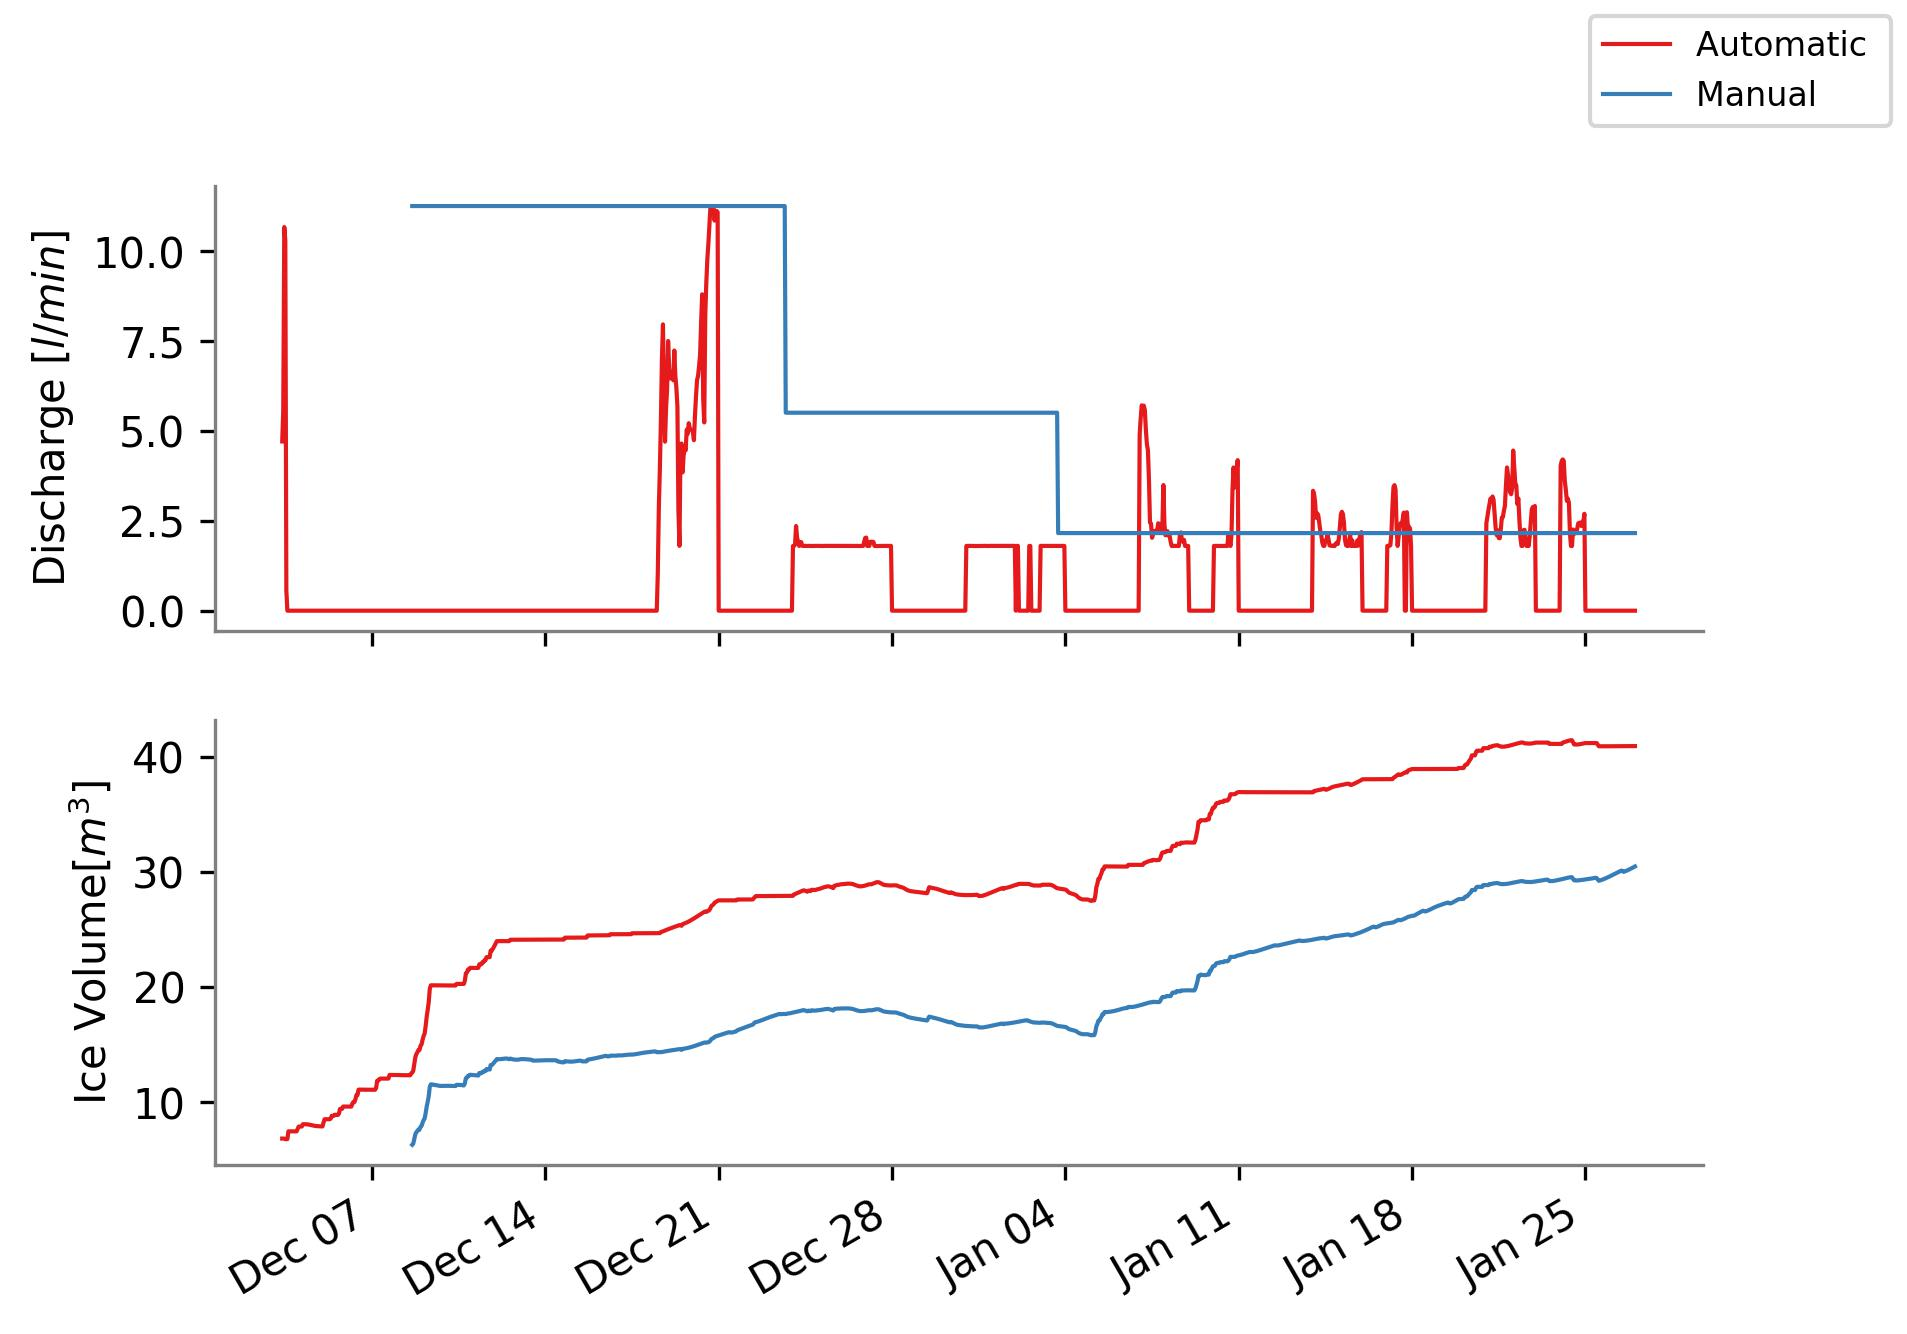
\includegraphics[width=\linewidth]{Figures/autovsmanual.jpg}
	\end{center}
	\caption{Icestupa in Ladakh, India on March 2017 was 24 $m$ tall and contained around 3700 $m^3$
		of water. Picture Credits: Lobzang Dadul}
	\label{fig:old_icestupa}
\end{figure}

\subsection{Validation}

\section{Discussion}

\section{Conclusions}

\section{Appendix}

\end{document}
